\documentclass[11pt]{article}
\usepackage{fullpage}
\usepackage{graphicx}
\usepackage{amsmath}
\usepackage{wasysym}
\usepackage{hyperref}
\usepackage{comment}
\usepackage{pdfpages}
\hypersetup{colorlinks=true, linkcolor=blue, bookmarks=true}

\newtheorem{remark}{Remark}
\newtheorem{example}{Example}
\newcommand{\eat}[1]{}
\begin{document}



\title{Web Information Retrieval (67782)\\ Ex2: Index Construction}
\date{}

\maketitle
\noindent {\bf Submitted by: Daniel Kerbel (CSE: danielkerbel, ID: ***REMOVED***)}

\section{Index creation runtime}

The computer which was used has the following specifications:

\begin{itemize}
	\item OS: Windows 10 64-bit
	\item CPU: Intel i5-7300 HQ at 2.5-3.5GHz
	\item RAM: 24GB of RAM, only allocated 1GB to the Java process
	\item Storage: The data-set was stored on a 7200 RPM external hard drive
\end{itemize}

The dataset is the entire \href{https://snap.stanford.edu/data/web-Amazon.html}{1995-2013 Amazon Dataset} (the \texttt{all.txt} file) 
which has the following statistics:

\begin{description}
	\item[Number of products] 34,686,770
	\item[Raw size] 35,781,618,251 bytes
	\item[Total amount of tokens] 2,909,591,866
	\item[Number of unique tokens] 413,742,857
\end{description}

Index creation was implemented using the SPIMI algorithm, and I've split the measurement into two stages:

\begin{itemize}
	\item Time taken by the "invert" stage (including parsing), where many temporary indices are created
	\item Time taken to merge all indices and create the final index
\end{itemize}

And the results are summarized by the following plot:

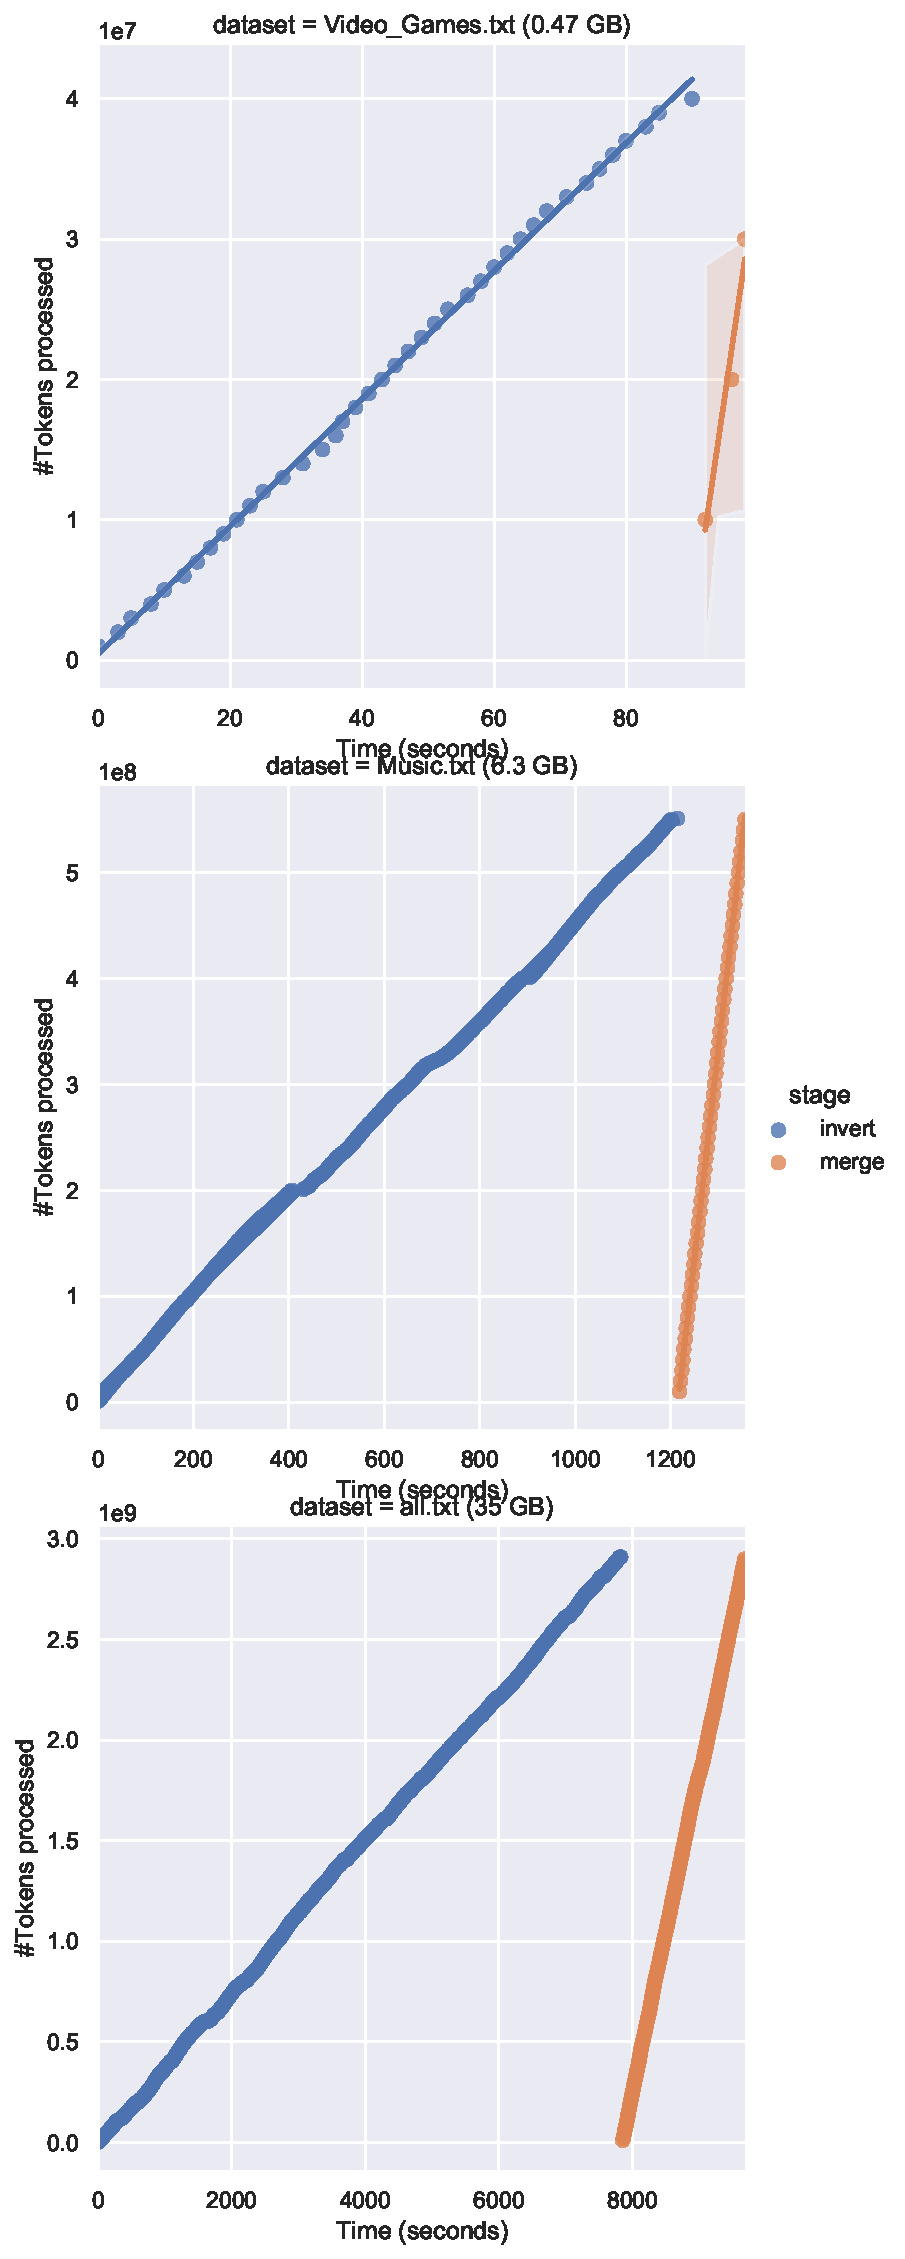
\includegraphics{runtime.pdf}


The invert stage also included IO for filling the "compact storage" which includes reviews metadata (which is just filled sequentially as
we encounter new documents, and doesn't require any sorting or special processing).
Not included is the time taken to sort productID - docID pairs, containing the lowest \& highest review IDs per product.
I've actually implemented this via an external sorting algorithm, but as it turns out, only 1 block was needed(the sort was performed entirely within memory), and finished in a couple seconds.

In total, it took about 8886 seconds to index this dataset, giving us a throughput of \textbf{4 MBps}

\section{Disk usage}

During the invert stage, 101 temporary indices were created, each taking around ~80-83 MB, and using a total of 8.35 GB, as summarized by the following plot:

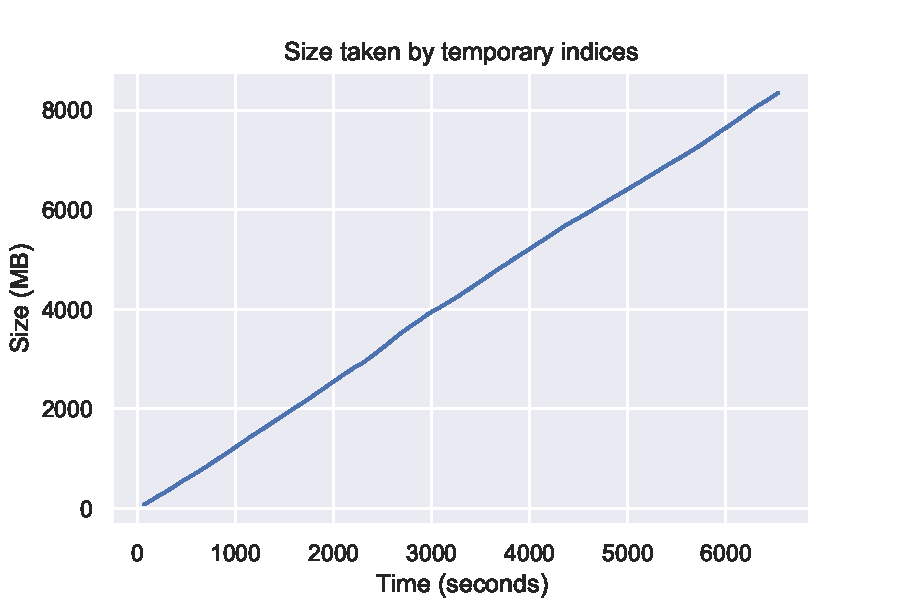
\includegraphics{diskusage.pdf}

Therefore, during the invert stage, we need a total of 44.13 GB \footnote{In theory, we could use less if we split the input file, as we only go over
	the input file once}, which means a $23\%$ overhead during index creation.

After merging, the final index takes \textbf{8.47 GB}. This means that during merging, we use a total of 16.82 GB (adding up the temporary and final indices,
but omitting the input files as they aren't needed at this point)



\end{document}
